\documentclass[11pt]{article}
\usepackage{graphicx}
\usepackage{hyperref}
\usepackage{float}
\title{Hopefully Self Driving Toy Car}
\author{Francesco Saverio Zuppichini, Alessia Ruggeri and Hanka Fazlic}
\begin{document}
\maketitle
%Title of your project
%Introduction / motivating scenario
%Prototype description that may include:
%Potential architecture / block diagram 
%Needed hardware components (e.g., sensors and actuators)
%Code to be written (e.g., Arduino code that supports WiFi connection)
\section{Introduction}
An autonomous car is a vehicle that is capable of sensing its environment and navigating without human input. Due to the advance in Machine Learning, Deep Learning, and hardware, in the last few years, lots of big companies, Tesla, Uber, and Google, started to test on the field self-driving car with success. 

Moreover, due to recent tragedy \footnote{http://www.bbc.com/news/world-us-Canada-43497364}, understanding this how the technology works and interact with the ambient is even more important. 

Normally, an autonomous car uses a wide array of sensors, from cameras around the car to LIDAR \footnote{https://en.wikipedia.org/wiki/Lidar}. The vehicle must be able to understand the surrounding, e.g. when a traffic light is red, as well as predict when it needs to act to avoid a dangerous situation. 

Our project aims to understand the dynamics of a self-driving car in a controlled test environment using a toy vehicle with only a frontal camera pointing the fake road created using two color lines. 

\section{Prototype}
Our toy car will be equipped with a cardboard computing, such as a raspberry pi, with a trained Neural Network in order to predict the steering angle only from the image from the camera. If during developer, we notice a high lag between input and prediction then the model will be placed on a server and the result streamed from the pi in order to reduce the lag.

Moreover, the on-board computer should be also able to control the wheels of the car. To keep things simple, we decide to go with a car model similar to the one showed in Figure \ref{fig: little_car}.

\begin{figure}[H]
\centering
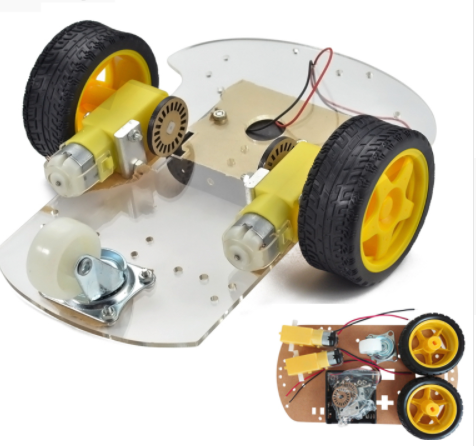
\includegraphics[scale=0.5]{images/little_car}
\caption{\href{https://it.aliexpress.com/item/Motor-Smart-Robot-Car-Chassis-Kit-Speed-Encoder-Battery-Box-2WD-For-Arduino-Free-Shipping/32766175672.html?spm=a2g0y.search0104.3.127.1fe64471Nd8YgA&ws_ab_test=searchweb0_0,searchweb201602_2_10152_10151_10065_10068_10344_10342_10343_10340_10341_10696_10084_10083_10618_10307_10134_5711215_10313_10059_10534_100031_10103_10624_10623_10622_10621_10620,searchweb201603_25,ppcSwitch_7&algo_expid=3450aa2c-e521-4594-a0c1-4bf8782da265-18&algo_pvid=3450aa2c-e521-4594-a0c1-4bf8782da265&priceBeautifyAB=0}{small car}}	
\label{fig: little_car}
\end{figure}
This small car has only two motors to control the two wheels, so in order to steer we need to stop one wheel while the other is running.

The road will be simulated using some colored tape, as showed in the following Figure
\begin{figure}[h]
\centering
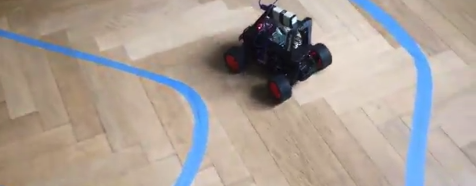
\includegraphics[width=\linewidth]{images/road}
\caption{Fake road on parquet}
\end{figure}
The brain of our vehicle is the onboard computer that, not only is responsible to actually turn on the motors, but also to calculate the prediction. 
Formally, the car will be equipped with a camera, then at each time $t$ the frame $f_t$ will be fed, probably after some preprocessing (e.g. convert the image to greyscale), to a neural network that will output the steering angle prediction in order to maintain the car on-road.

While building the model may be an not challenging task, due to the already existing material online, gathering the data to train it is the other story. Usually, in real life scenario, huge dataset of the real human person driving car can be used, but we think that in our case they may not work well. 

One trivial solution that works for other people, is to manually move the car simulating a correct run while recording. Then, use the frames as the training set.

Still, we will need to find out the best ration between skip frames and make trace out of them. 
If everything works and we will have time, an infrared sensor can be placed in front of the vehicle in order to avoid obstacles.

\section{Hardware components}
\begin{itemize}
	\item \href{https://it.aliexpress.com/item/Motor-Smart-Robot-Car-Chassis-Kit-Speed-Encoder-Battery-Box-2WD-For-Arduino-Free-Shipping/32766175672.html?spm=a2g0y.search0104.3.127.1fe64471Nd8YgA&ws_ab_test=searchweb0_0,searchweb201602_2_10152_10151_10065_10068_10344_10342_10343_10340_10341_10696_10084_10083_10618_10307_10134_5711215_10313_10059_10534_100031_10103_10624_10623_10622_10621_10620,searchweb201603_25,ppcSwitch_7&algo_expid=3450aa2c-e521-4594-a0c1-4bf8782da265-18&algo_pvid=3450aa2c-e521-4594-a0c1-4bf8782da265&priceBeautifyAB=0}{Car} 
	\item \href{https://it.aliexpress.com/item/Free-Shipping-5MP-New-Raspberry-pi-2-Camera-Module-Board-REV-1-3-5MP-Webcam-Video/32522482332.html?spm=a2g0y.search0104.3.2.7cbac3ebsWO1vu&ws_ab_test=searchweb0_0,searchweb201602_2_10152_10151_10065_10068_10344_10342_10343_10340_10341_10696_10084_10083_10618_10307_5711220_10134_10313_10059_10534_100031_10103_10624_10623_10622_10621_10620,searchweb201603_25,ppcSwitch_7&algo_expid=51db4307-aeb9-446b-a5ce-1ab07e41e291-0&algo_pvid=51db4307-aeb9-446b-a5ce-1ab07e41e291&priceBeautifyAB=0}{pi camera}
	\item \href{https://shop.pimoroni.com/collections/raspberry-pi/products/raspberry-pi-3-b-plus}{Raspberry Pi}
	\item Tape
	\item A motor driver, something like the L293 
	
\end{itemize}
\end{document}
